\documentclass[a4paper,12pt]{article}
\usepackage[T1]{fontenc}
\usepackage[utf8]{inputenc}
\usepackage{lmodern}
\usepackage[french]{babel}
\usepackage{url,csquotes}
\usepackage[hidelinks,hyperfootnotes=false]{hyperref}
\usepackage{enumitem}
\usepackage{amsmath}
\usepackage{graphicx}

\usepackage{caption}
\usepackage{subcaption}
\usepackage{float}


\title{Quantum Monte Carlo algorithm for spins systems}
\author{Etienne \bsc{Camphuis}}


\begin{document}
	\begin{titlepage}
		\begin{center}
			\textsc{\Large Physique numérique}\\[1.5cm]
			
			{ \large \bfseries Algorithme de Monte Carlo pour les systèmes de spins\\[0.3cm] }
		\begin{abstract}
			On modélise une chaîne de spin quantique grâce au modèle XXZ, c'est à dire avec l'hamiltonien suivant:
			\begin{equation}
				\centering
				H =  J_x \sum_{i} ( S_i^xS_{i+1}^x + S_i^yS_{i+1}^y ) + J_z \sum{i} S_i^zS_{i+1}^z
			\end{equation}
			Pour trouver l'énergie moyenne du système à température donnée, on utilise un algorithme de Monte Carlo "quantique" vu en cours, l'intégrale des chemins de Feynman. Cette fois-ci, la représentation est en 2D et suit des règles précises de validité pour les configurations. \\
			Le but du projet est de coder, d'appliquer et de comparer deux types d'algorithmes, qui proposent des mouvements différents. Le premier a une approche assez intuitive de mouvements locaux. Le deuxième propose des mouvements globaux impressionants, qui permettent de réduire le temps d'autocorrélation et le nombre de mesures drastiquement. Ce type de mouvement, appelés \emph{mouvement de boucles}, est utilisé dans bien d'autres modélisations physiques. \\
			La difficulté du projet réside dans l'écriture de la \emph{balance détaillée} et des poids, qui peuvent être négatifs, a contrario du spin \og classique \fg.
			\begin{figure}[H]
				\centering
				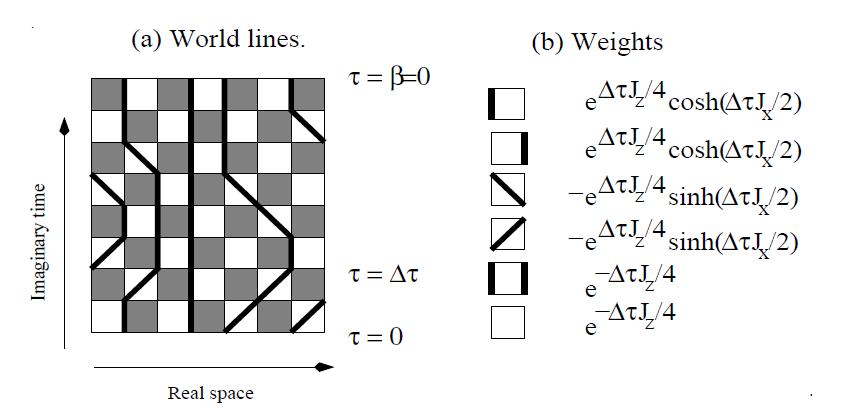
\includegraphics[width=8cm]{pathintegral.png}
				\caption{Exemple de configuration et poids associés}
			\end{figure}
		\end{abstract}
		\vfill
		\begin{minipage}{0.7\textwidth}
			\centering
			Etienne \textsc{Camphuis}\\
			Barthélémy \textsc{Meynard Piganeau} \\
		\end{minipage}
		\end{center}
	\end{titlepage}

\end{document}